\clearpage
\section{First look at 13 TeV data\label{app:firstlook13TeV}}

Following the first of several commissioning collisions at 13 TeV, it is possible to begin exercising
the workflow of the analysis in preparation for further data acquisition. 
It should be noted that the detector conditions during the first collisions had no magnetic field, which as a result prevented access to physics objects computed with the full detector.

Examples of the variables of interest, in particular electron based quantities from a certified {\textit{EGamma}} stream at 13 TeV, can be seen in Figs.~\ref{fig:firstlook_13TeV}.
These preliminary distributions are compared to {\textit{RelVal Minimum Bias}} MC at 0T.
The integrated luminosity of the data corresponds to 4.9 nb$^{-1}$ and the MC has been weighted to match the integral of data. 


\begin{figure}[H]
 \begin{center}  
  \subfigure[electron $\eta$]{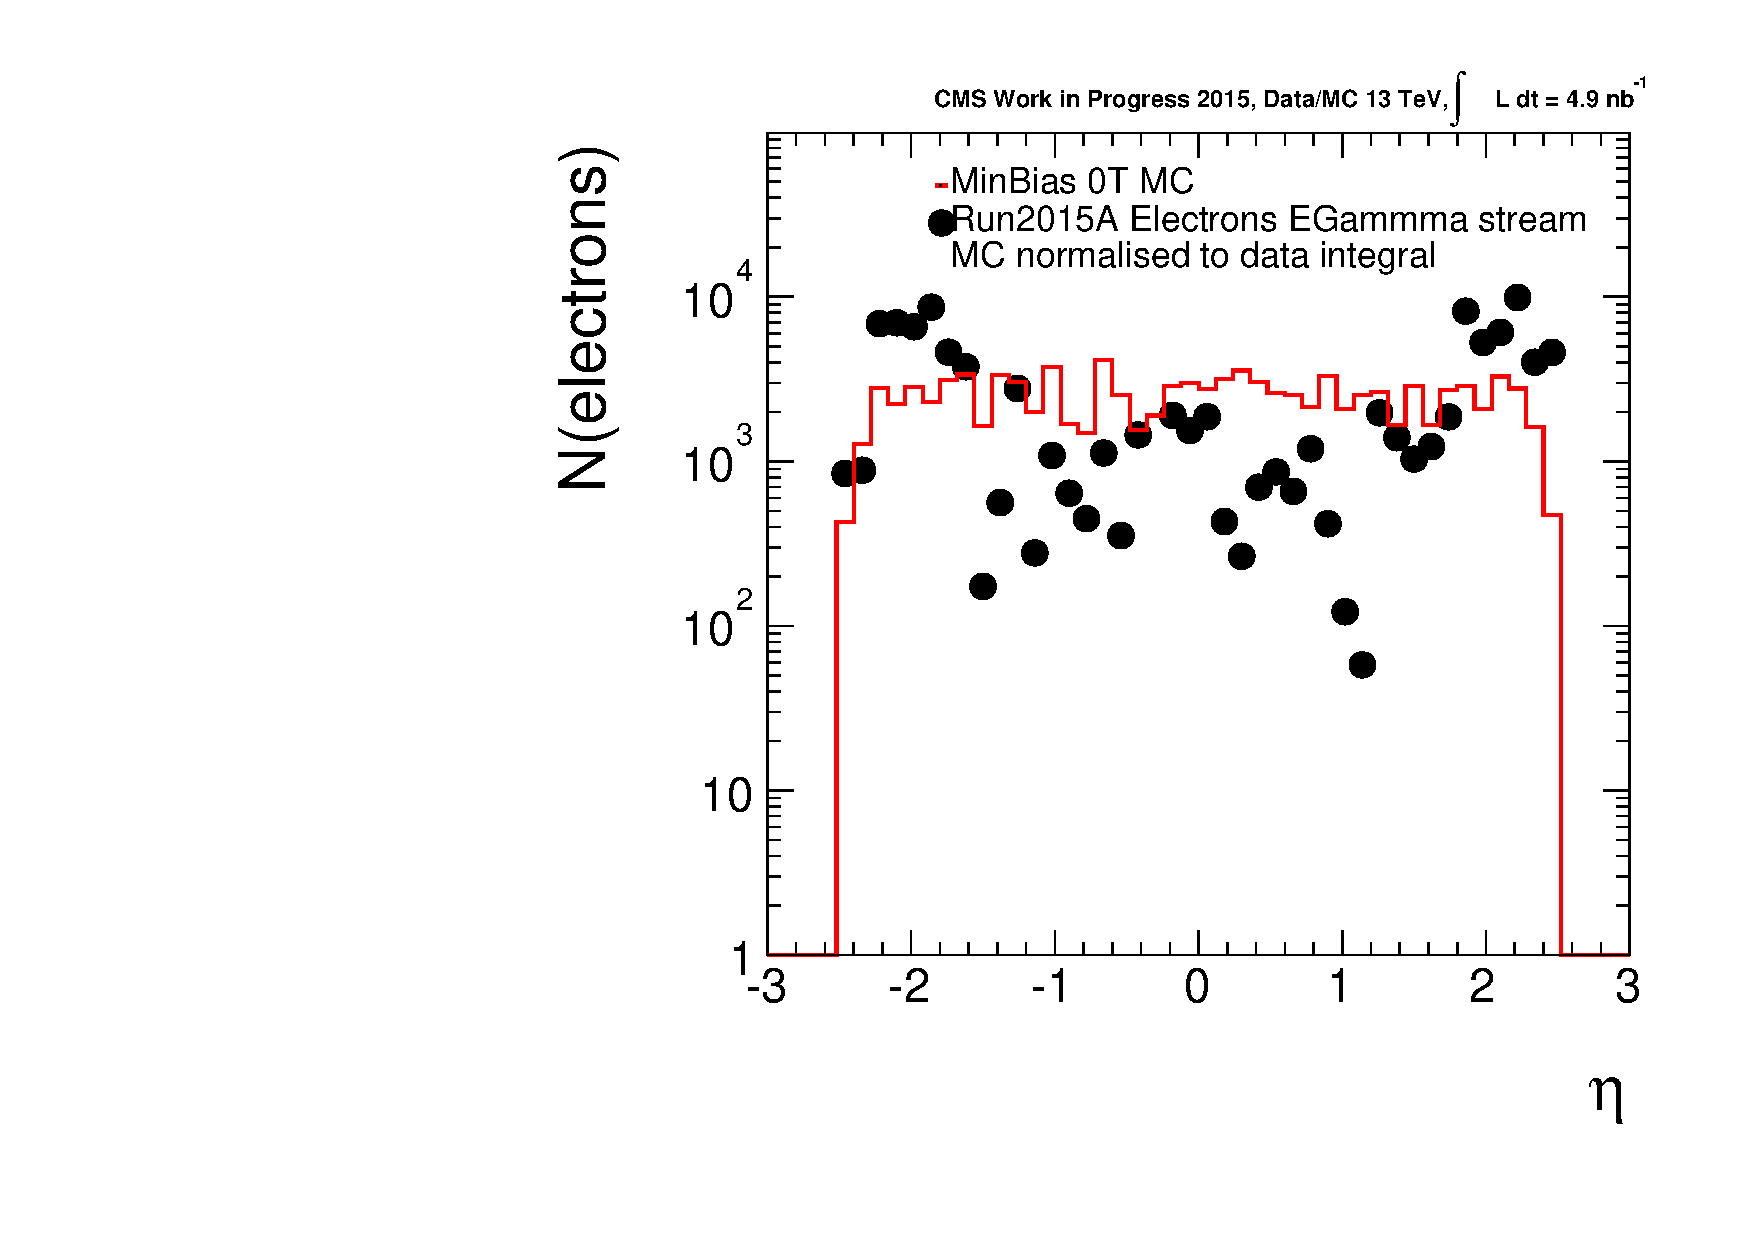
\includegraphics[width=0.5\textwidth]{figures/FirstLook_13TeV/hDataVsMC_Data_EleEta.pdf}} ~~
  \subfigure[electron $\phi$]{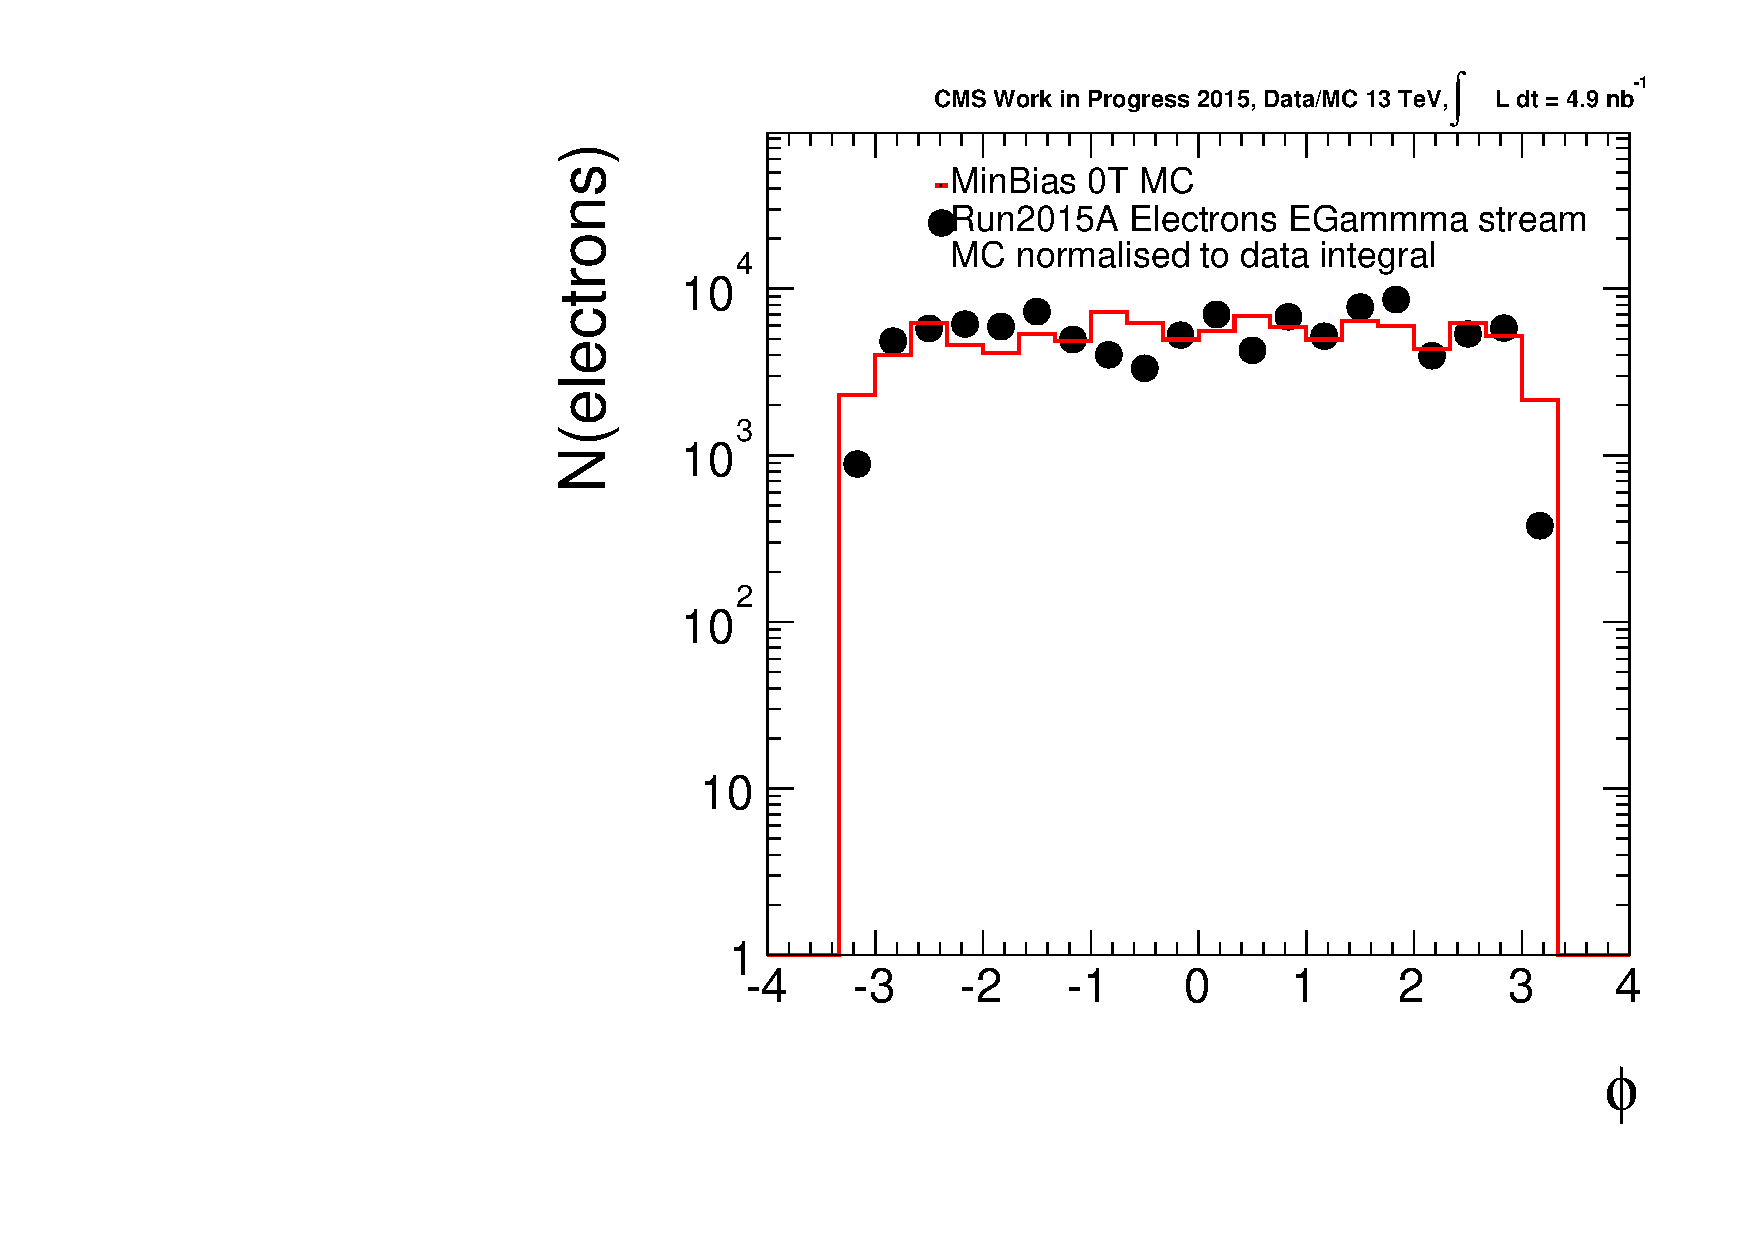
\includegraphics[width=0.5\textwidth]{figures/FirstLook_13TeV/hDataVsMC_Data_ElePhi.pdf}} ~~ \\
  \subfigure[electron $\frac{H}{E}$]{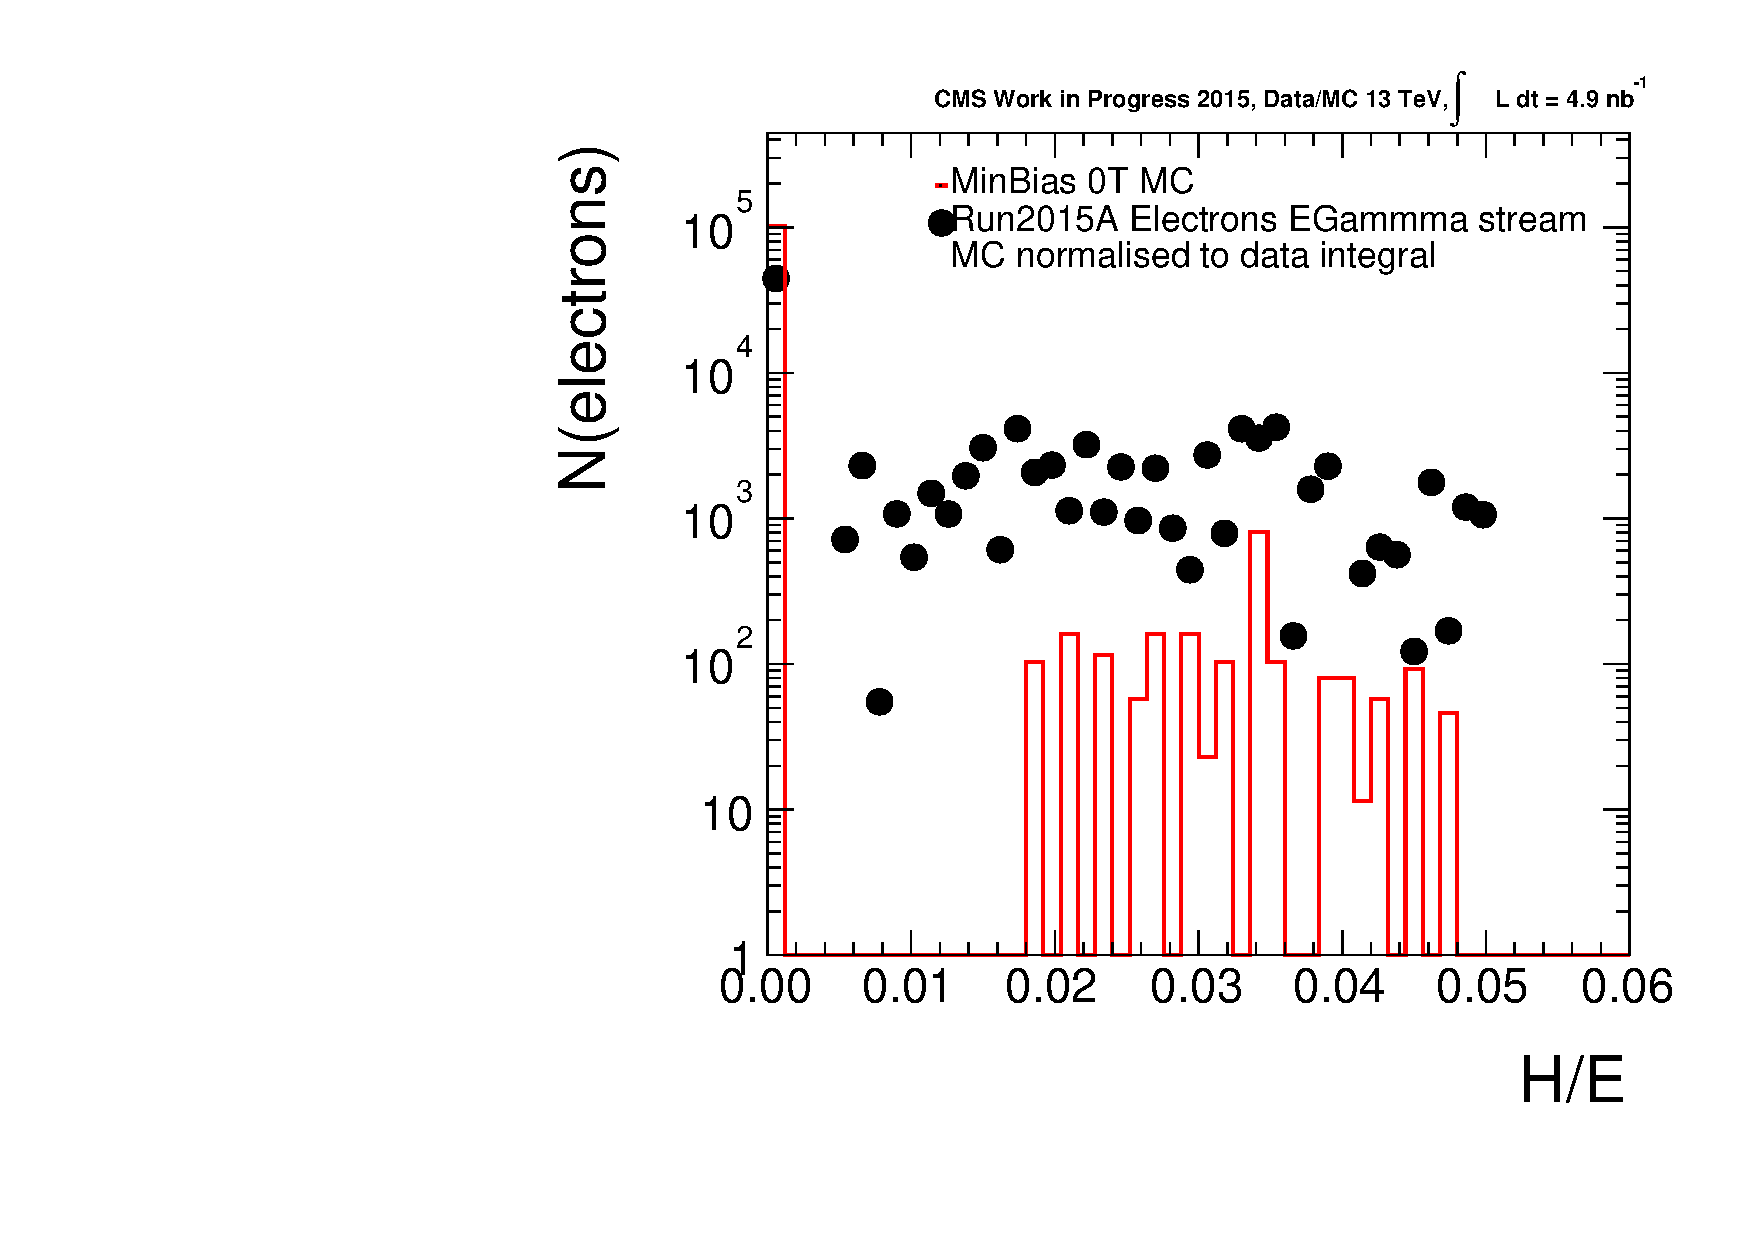
\includegraphics[width=0.5\textwidth]{figures/FirstLook_13TeV/hDataVsMC_Data_EleHoverE.pdf}} ~~
  \subfigure[no. electrons]{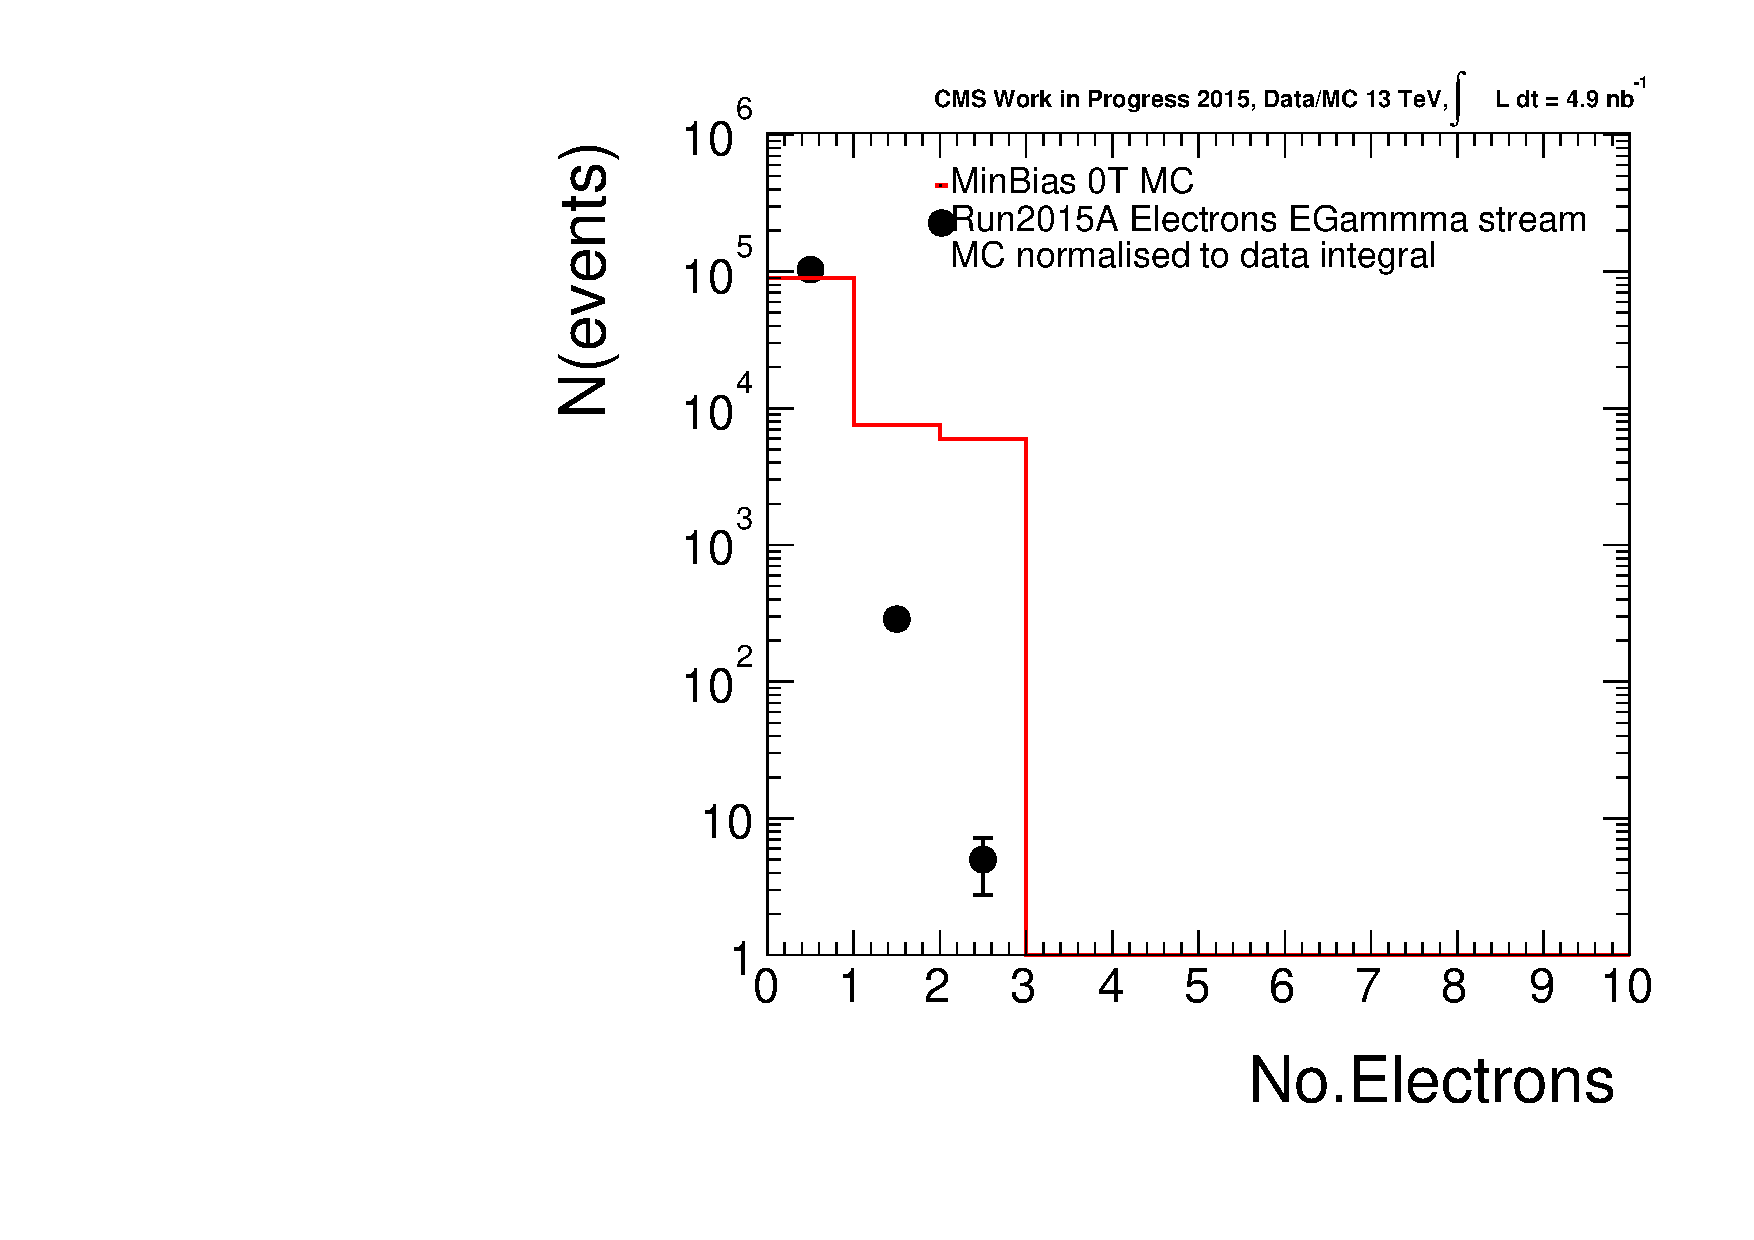
\includegraphics[width=0.5\textwidth]{figures/FirstLook_13TeV/hDataVsMC_Data_NElec.pdf}} \\
  \caption{First look at Data / MC at 13 TeV}
  \label{fig:firstlook_13TeV}
 \end{center}
\end{figure}          
